
\section{Classification}
\textbf{Average classification (generalization) error}\\
$R(\hat{f}) = \mathbb{E}_{x,y}\mathbb{I}_{y \neq sign \hat{f}(x)}$ (the surrogate loss function is neither convex nor continuous, so it could not be used for minimizing training error!) \\
\textbf{Convexify the surrogate losses}\\
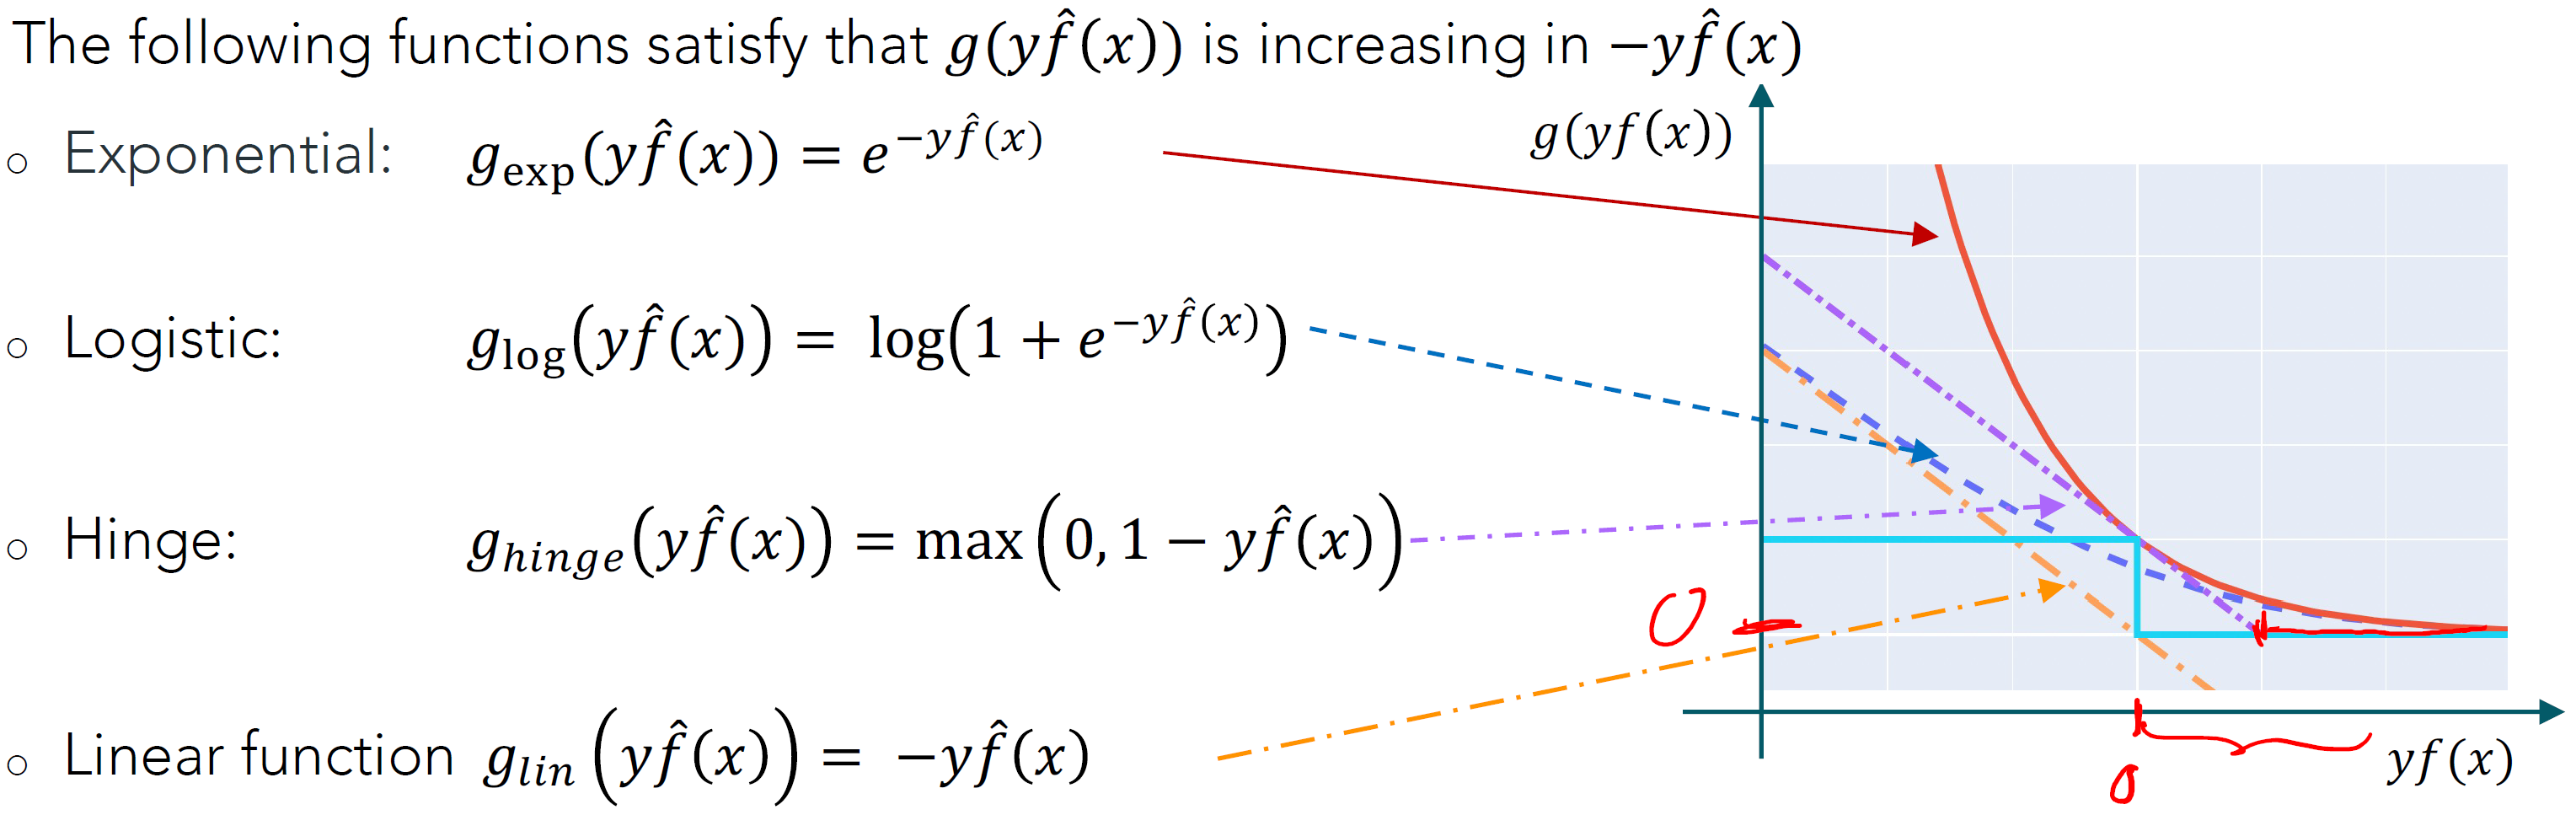
\includegraphics[width=\linewidth]{pics/figure5.PNG} 
\textbf{Logistic loss}: binary classification\\
$\ell_{log}(\hat{f}(x), y) = log(1 + e^{-y\hat{f}(x)}) = -log(Prob(Y=y|x)$ (condi. log-likeli.  param. by $\hat{f}(x) = (\hat{f}_1(x), \cdots, \hat{f}_k(x))$ via $p_i = softmax(\bar{f}_i) = \frac{exp(\alpha \Bar{f_i})}{ \sum_{j=1}^K exp(\alpha \Bar{f_j})}, \alpha > 0$) \\
\textbf{Cross-entropy loss}: multi-class classification see 10.3
\textbf{Maximum-Margin and SVM}: \\
Motivation: for linearly separable data, \textbf{no unique solution} for the training loss by using the logistic loss. \\
General formulation of the optimization problem: $w_{MM} = \arg \max_{||w||_2 = 1} margin(w)$ where margin$(w)=\min_{i} y_i\langle  w , x_i \rangle$  \\
\textbf{Soft-Margin SVM} \\
If data is not linearly separable (constraints that allow some "slack" in the constraint):\\
%\begin{equation}
$\min_{w,\xi} \frac{1}{2}||w||^2 + \lambda\sum_{i} \xi_{i}$ 
%\end{equation}
s.t. ${y_i}{w^T}{x_i} \geq 1 - \xi_{i}, {\xi_{i} \geq 0}$ for all i = 1, ...., n\\
converted to ($l_2$ penalized hinge loss):\\
%\begin{equation}
$\min_{w} \frac{1}{2}||w||^2 + \lambda\sum_{i} \max(0, 1-{y_i}{w^T}{x_i})$\\
%\end{equation}

\textbf{Area under the ROC (AUROC)}:\\
Ideal curve: higher TPR (y-axis) \& lower FPR (x-axis)\\
\textbf{F1-score}:$F_1 score = \frac{2}{\frac{1}{recall} + \frac{1}{precision}}$ (Why not average? For both recall and precision to be large) \\
\textbf{Accuracy:} $\operatorname{Acc}(y,\hat{y})=\frac{1}{n_{\mathrm{samples}}}\sum_i 1(\hat{y}_i=y_i)$ \\
\textbf{Recall \& Precision}
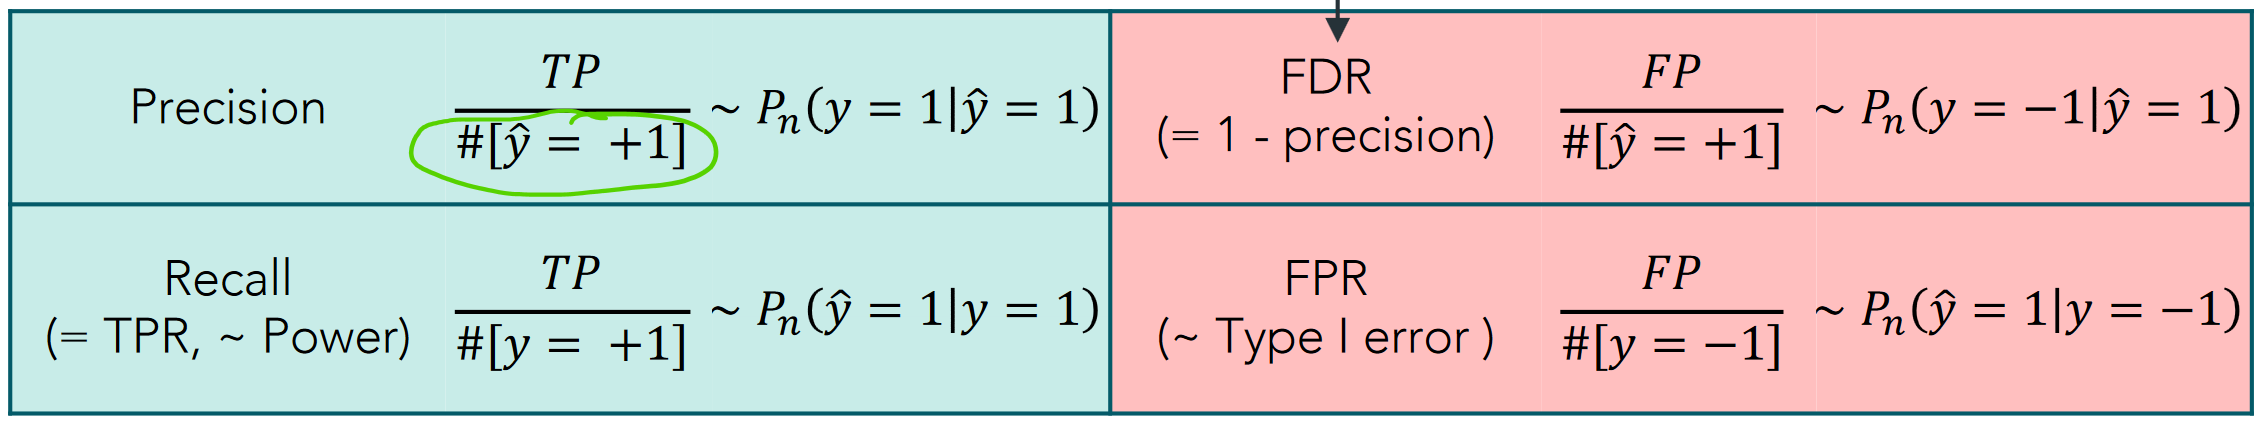
\includegraphics[width=\linewidth]{pics/figure6.PNG} \\
\textbf{Other metrics in practice}: \\
1. Worst group error (related to group fairness);\\
2. Advesarial pertubations (robustness againts data transformations);\qquad
3. Distribution shifts on the inputs (same label but data looks different)



